\documentclass[12pt,a4paper]{article}
\usepackage[affil-it]{authblk}
\usepackage{amsthm}
\usepackage{amssymb}
\usepackage{amsmath}
\usepackage{listings}
\usepackage{graphicx}
\usepackage{pgfplots}
\usepackage{float}
\usepackage{xcolor}
\usepackage{hyperref}
       
\usepackage[
  backend=biber,
  style=alphabetic,
  sorting=anyt,
  minnames=3,
  minalphanames=3
]{biblatex}

\hypersetup{
    colorlinks=true,
    citecolor=blue,
    linkcolor=black,
    urlcolor=blue,
    pdftitle={NP-Completeness Steiner Tree},
}

\newtheorem{definition}{Definition}
\newtheorem{problem}{Problem}
\newtheorem{claim}{Claim}

\definecolor{sapRed}{HTML}{6f0a19}
\definecolor{sapBlue}{HTML}{006778}

\newcommand{\curlyquotes}[1]{\textquotedblleft #1\textquotedblright}
\newcommand{\abs}[1]{\left|#1\right|}
\newcommand{\abk}[1]{\left\langle#1\right\rangle}

\addbibresource{./references.bib}

\begin{document}

    \title{NP-Completeness of the Steiner Tree Problem}
    \author{Simone Bianco}
    \affil{Sapienza Università di Roma, Italy}
    \date{\today}

    \maketitle

    \abstract{The Steiner tree (ST) problem is an optimization problem in graph theory with applications in network design and computational biology. This essay proves the $\mathsf{NP}$-Completeness for the decision version of the problem in undirected graphs by showing membership in $\mathsf{NP}$ and constructing a polynomial-time reduction from the $\mathsf{NP}$-Complete Exact Cover by 3-Sets (X3C) problem}

    \tableofcontents
    \newpage

    \section{The Steiner tree problem}

    The Steiner tree problem is an optimization problem that arises in various fields, including network design, computational biology, and VLSI design. While there are many formulations of this problem, they all require to find an optimal interconnection for a given set of objects, called \textit{terminals}, for a predefined objective function, which usually asks to minimize the length of such interconnections. This problem has many applications, especially when planning a connecting structure among different terminal points to minimize overall cost or distance. \cite{shortest_network}
    
    The usual formulation of this problem is achieved through graphs, where each node of the graph acts as an connection point that defines interconnections through edges. The terminals are also represented as nodes of the graph. A Steiner tree must cover all the designed terminal nodes.
    
    \begin{definition}
        Given a graph $G$ and a subset of nodes $S \subseteq V(G)$, called \textit{terminal set}, a Steiner tree (ST) for $S$ in $G$ is a sub-tree $T$ such that covers all the nodes of $S$, i.e. $S \subseteq V(T)$.
    \end{definition}

    In particular, we notice that, by definition, a Steiner tree can also contain nodes that aren't part of the terminal set. These nodes are called \textit{Steiner points}. The Steiner tree problem asks to find an ST for a given set of terminal nodes with the lowest possible number of edges.

    \begin{problem}
        Given a graph $G$ and a subset of nodes $S \subseteq V(G)$, find a Steiner tree with the minimum number of edges.
    \end{problem}

    \begin{figure}[H]
        \centering

        \resizebox{0.5\textwidth}{!}{
            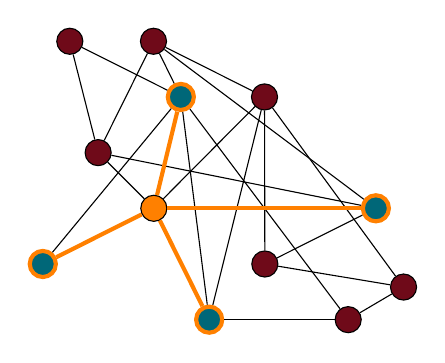
\begin{tikzpicture}[]
                \node[circle, draw, fill=sapRed] (1) [] {};
                \node[circle, draw, orange, line width=1.5, fill=sapBlue] (2) [above left of = 1, xshift=50] {};
                \node[circle, draw, fill=orange] (3) [below right of = 1, xshift=0] {};
                \node[circle, draw, fill=sapRed] (4) [above left of = 2, xshift=-20] {};
                \node[circle, draw, fill=sapRed] (5) [above right of = 2, xshift=-30] {};
                \node[circle, draw, orange, line width=1.5, fill=sapBlue] (6) [below left of = 3, xshift=-20] {};
                \node[circle, draw, fill=sapRed] (7) [below right of = 3, xshift=20] {};
                \node[circle, draw, fill=sapRed] (8) [below right of = 7, xshift=10] {};
                \node[circle, draw, orange, line width=1.5, fill=sapBlue] (9) [below left of = 7, xshift=0] {};
                \node[circle, draw, orange, line width=1.5, fill=sapBlue] (10) [above right of = 7, xshift=20] {};
                \node[circle, draw, fill=sapRed] (11) [above right of = 1, xshift=40] {};
                \node[circle, draw, fill=sapRed] (12) [below of = 10, xshift=10] {};

                \path[every node/.style={font=\sffamily\small}]
                    (1) edge (10)
                    (2) edge (9)
                    (4) edge[] (1)
                    (5) edge[] (2)
                    (6) edge[color=orange, line width=1.5] (3)
                    (1) edge[] (3)
                    (3) edge[color=orange, line width=1.5] (2)
                    (2) edge (6)
                    (3) edge[color=orange, line width=1.5] (9)
                    (4) edge[] (2)
                    (5) edge (10)
                    (8) edge[] (2)
                    (1) edge (5)
                    (8) edge[] (9)
                    (11) edge[] (7)
                    (11) edge[] (3)
                    (11) edge (5)
                    (11) edge[] (12)
                    (11) edge (9)
                    (12) edge (7)
                    (12) edge[] (8)
                    (3) edge[color=orange, line width=1.5] (10)
                    (10) edge (7)
                ;
            \end{tikzpicture}
        }
            
        \caption{Minimum Steiner tree for the given terminals (blue nodes)}
    \end{figure}

    An interesting thing to notice is that this formulation of the Steiner tree problem acts as a generalization two well-known combinatorial optimization problems: the \textit{Shortest Path problem} and the \textit{Minimum Spanning Tree problem}. In particular, finding the minimum Steiner tree on two terminals is equivalent to finding the shortest path between them. When all vertices in the graph are terminals, instead, the problem becomes equivalent to finding the minimum spanning tree of the graph.

    
    \begin{figure}[H]
        \centering

        \resizebox{1\textwidth}{!}{
            \begin{tabular}{ccc}
                \begin{tabular}{c}
                    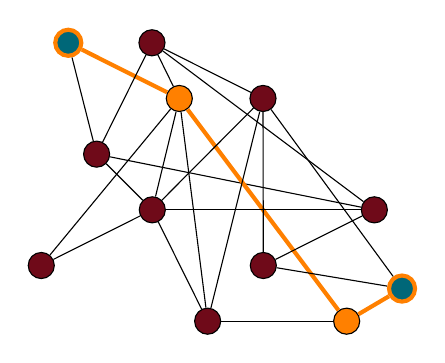
\begin{tikzpicture}
                        \node[circle, draw, fill=sapRed] (1) [] {};
                        \node[circle, draw, fill=orange] (2) [above left of = 1, xshift=50] {};
                        \node[circle, draw, fill=sapRed] (3) [below right of = 1, xshift=0] {};
                        \node[circle, draw, orange, line width=1.5, fill=sapBlue] (4) [above left of = 2, xshift=-20] {};
                        \node[circle, draw, fill=sapRed] (5) [above right of = 2, xshift=-30] {};
                        \node[circle, draw, fill=sapRed] (6) [below left of = 3, xshift=-20] {};
                        \node[circle, draw, fill=sapRed] (7) [below right of = 3, xshift=20] {};
                        \node[circle, draw, fill=orange] (8) [below right of = 7, xshift=10] {};
                        \node[circle, draw, fill=sapRed] (9) [below left of = 7, xshift=0] {};
                        \node[circle, draw, fill=sapRed] (10) [above right of = 7, xshift=20] {};
                        \node[circle, draw, fill=sapRed] (11) [above right of = 1, xshift=40] {};
                        \node[circle, draw, orange, line width=1.5, fill=sapBlue] (12) [below of = 10, xshift=10] {};

                        \path[every node/.style={font=\sffamily\small}]
                            (1) edge (10)
                            (2) edge (9)
                            (4) edge[] (1)
                            (5) edge[] (2)
                            (6) edge[] (3)
                            (1) edge[] (3)
                            (3) edge[] (2)
                            (2) edge (6)
                            (3) edge[] (9)
                            (4) edge[color=orange, line width=1.5] (2)
                            (5) edge (10)
                            (8) edge[color=orange, line width=1.5] (2)
                            (1) edge (5)
                            (8) edge[] (9)
                            (11) edge[] (7)
                            (11) edge[] (3)
                            (11) edge (5)
                            (11) edge[] (12)
                            (11) edge (9)
                            (12) edge (7)
                            (12) edge[color=orange, line width=1.5] (8)
                            (3) edge[] (10)
                            (10) edge (7)
                        ;
                    \end{tikzpicture}
                \end{tabular}

                &\quad&

                \begin{tabular}{c}
                    
                    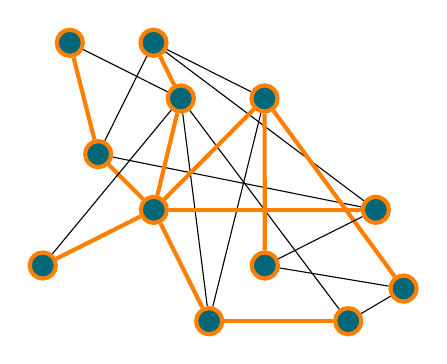
\begin{tikzpicture}
                        \node[circle, draw, orange, line width=1.5, fill=sapBlue] (1) [] {};
                        \node[circle, draw, orange, line width=1.5, fill=sapBlue] (2) [above left of = 1, xshift=50] {};
                        \node[circle, draw, orange, line width=1.5, fill=sapBlue] (3) [below right of = 1, xshift=0] {};
                        \node[circle, draw, orange, line width=1.5, fill=sapBlue] (4) [above left of = 2, xshift=-20] {};
                        \node[circle, draw, orange, line width=1.5, fill=sapBlue] (5) [above right of = 2, xshift=-30] {};
                        \node[circle, draw, orange, line width=1.5, fill=sapBlue] (6) [below left of = 3, xshift=-20] {};
                        \node[circle, draw, orange, line width=1.5, fill=sapBlue] (7) [below right of = 3, xshift=20] {};
                        \node[circle, draw, orange, line width=1.5, fill=sapBlue] (8) [below right of = 7, xshift=10] {};
                        \node[circle, draw, orange, line width=1.5, fill=sapBlue] (9) [below left of = 7, xshift=0] {};
                        \node[circle, draw, orange, line width=1.5, fill=sapBlue] (10) [above right of = 7, xshift=20] {};
                        \node[circle, draw, orange, line width=1.5, fill=sapBlue] (11) [above right of = 1, xshift=40] {};
                        \node[circle, draw, orange, line width=1.5, fill=sapBlue] (12) [below of = 10, xshift=10] {};

                        \path[every node/.style={font=\sffamily\small}]
                            (1) edge (10)
                            (2) edge (9)
                            (4) edge[color=orange, line width=1.5] (1)
                            (5) edge[color=orange, line width=1.5] (2)
                            (6) edge[color=orange, line width=1.5] (3)
                            (1) edge[color=orange, line width=1.5] (3)
                            (3) edge[color=orange, line width=1.5] (2)
                            (2) edge (6)
                            (3) edge[color=orange, line width=1.5] (9)
                            (4) edge[] (2)
                            (5) edge (10)
                            (8) edge[] (2)
                            (1) edge (5)
                            (8) edge[color=orange, line width=1.5] (9)
                            (11) edge[color=orange, line width=1.5] (7)
                            (11) edge[color=orange, line width=1.5] (3)
                            (11) edge (5)
                            (11) edge[color=orange, line width=1.5] (12)
                            (11) edge (9)
                            (12) edge (7)
                            (12) edge[] (8)
                            (3) edge[color=orange, line width=1.5] (10)
                            (10) edge (7)
                        ;
                    \end{tikzpicture}                
                \end{tabular}
            \end{tabular}
        }

        \caption{The ST problem on two nodes (left) and all nodes (right)}
    \end{figure}
    
    While both of these problems can be solved in polynomial time, the Steiner tree problem is significantly more challenging. In fact, the Steiner tree problem results to be \curlyquotes{intractable} unless $\mathsf{P} = \mathsf{NP}$. This is due to the $\mathsf{NP}$-Completeness of the decision version of this problem, which implies that the standard optimization variant is $\mathsf{NP}$-Hard \cite{np_complete}. The decision version of the problem is defined as follows.

    \begin{problem}
        Given a graph $G$, a subset of nodes $S \subseteq V(G)$ and an integer $k > 0$, determine if there is a Steiner tree for $S$ with at most $k$ edges.
    \end{problem}

    It's easy to see that this decision problem is a member of $\mathsf{NP}$, since the requested Steiner tree can act as a witness. In particular, we can verify a witness $T$ through this simple certification procedure, whose steps can all be done in time $O(\abs{V(G)} + \abs{E(G)})$:
    \begin{enumerate}
        \item Check that $T$ is a subgraph of $G$, i.e. that $V(T) \subseteq V(G)$ and $E(T) \subseteq E(G)$.
        \item Check that $T$ is a tree, i.e. that it contains no cycles
        \item Check that $T$ covers all the terminals, i.e. that $S \subseteq V(T)$
        \item Check that $T$ has at most $k$ edges, i.e. that $\abs{E(T)} \leq k$
    \end{enumerate}

    \section{The Exact Cover by 3-Sets problem}

    To show the $\mathsf{NP}$-Hardness of the Steiner tree problem, we have to find an $\mathsf{NP}$-Hard problem that can be reduced in polynomial time to it. Since the concept of Minimal Steiner tree reduces to the concept of \curlyquotes{terminal coverage}, it's easy to see that the former should be somehow related to the \textit{minimal set coverage problem}.

    Given an universe set $U = \{x_1, \ldots, x_n\}$ and a collection of subsets $\mathcal{C} = \{C_1, \ldots, C_m\}$ where $C_i \subseteq U$, a set cover of $U$ over $C$ is a sub-collection $\mathcal{C}^* \subseteq \mathcal{C}$ that covers $U$, that is $U = \bigcup_{C_i \in \mathcal{C}^*} C_i$. The Set Cover (SC) problem asks to find the minimum cardinality set cover.

    \begin{figure}[H]
        \[U = \{x_1, x_2, x_3, x_4, x_5, x_6, x_7\}\]
        \[C_1 = \{x_1, x_2, x_4, x_7\} \quad C_2 = \{x_1, x_3, x_5, x_6\} \quad C_3 = \{x_3, x_5, x_7\}\]

        \caption{Example of a set cover problem instance}
    \end{figure}
    
    Similarly to what we deed for the ST problem, the decision version of the set coverage problem would ask to decide if there is a set cover of at most $k$ subsets. Even though we can indeed convert the set cover problem to a \textit{terminal coverage} instance, we need still have some issues: any trivial Karp reduction, i.e. a poly-time reduction, from SC to ST has some counter-examples for which the minimal cover is mapped to a graph that contains cycles, which isn't a tree. 
    
    To force this constraint, we need a stronger variant of the set coverage problem, that being the \textit{exact cover} (XC) problem. This variant of the problem has one additional condition: the subsets inside the minimal cover must be pairwise disjoint, meaning that each element of $U$ lie only inside one of the subsets. In other words, we're asked to find a partition using the subsets of the given collection. Indeed, this variant of the problem fixes the previous issue, but there still is something to fix: we don't know how many edges the resulting Steiner tree must have. To fix this final issue, we use another stronger variant of the exact cover problem: the \textit{exact cover by 3-sets} (X3C) problem.

    This new problem has a third constraint: the universe set has $3q$ elements for some integer $q > 0$ and each of the subsets inside the collection has $3$ elements. The decision version of this problem, defined as follows, is $\mathsf{NP}$-Complete, where the hardness is obtained through a reduction from the 3D Matching problem.

    \begin{definition}
        Given a set $U = \{x_1, \ldots, x_{3q}\}$ and a collection of subsets $\mathcal{C} = \{C_1, \ldots, C_m\}$ such that $C_i \subseteq U$ and $\abs{C_i} = 3$, determine if there is a sub-collection $\mathcal{C}^* \subseteq  \mathcal{C}$ that is a partition of $U$.
    \end{definition}

    \section{Karp reduction from X3C to ST}

    After discussing why we chose the Exact Cover by 3-Sets problem as a candidate to show the $\mathsf{NP}$-Hardness of the ST problem, we're ready to give the polynomial time reduction. Given an instance $\abk{U,\mathcal{C}}$ of X3C, the reduction proceeds as follows:
    \begin{enumerate}
        \item For every subset $C_i \in \mathcal{C}$, we add a node $u_i$ in $G$.
        \item For every element $x_j \in U$, we add a node $v_i$ in $G$. For every $i \in [m]$, if $x_j \in C_i$ then we add the edge $(u_i, v_j)$ in $G$.
        \item We add a special node $z$ and an edge $(z, u_i)$ in $G$ for all $i \in [m]$.
        \item Let $S = \{z, x_1, \ldots, x_{3q}\}$.
        \item Return $\abk{G,S,4q}$.
    \end{enumerate}

    \noindent
    To better understand how the procedure works, the following X3C instance is transformed into the graph below it:
    \[U = \{x_1, x_2, x_3, x_4, x_5, x_6\}\]
    \[C_1 = {x_1, x_2, x_4} \quad C_2 = \{x_1, x_3, x_5\} \quad C_3 = \{x_3, x_5, x_6\} \quad C_4 = \{x_1, x_4, x_6\}\]

    \begin{figure}[H]
        \centering

        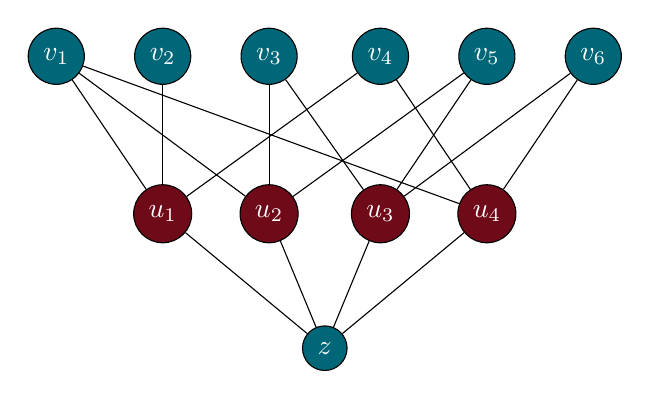
\begin{tikzpicture}
            \node[circle, draw, fill=sapBlue, text=white] (1) [] {$z$};
            \node[] (w) [above of = 1] {};

            \node[circle, draw, fill=sapRed, text=white] (2) [above left of = w] {$u_2$};
            \node[circle, draw, fill=sapRed, text=white] (3) [left of = 2, xshift = -10] {$u_1$};
            \node[circle, draw, fill=sapRed, text=white] (4) [above right of = w] {$u_3$};
            \node[circle, draw, fill=sapRed, text=white] (5) [right of = 4, xshift = 10] {$u_4$};

            \node[] (x) [above of = w] {};
            \node[] (y) [above of = x] {};

            \node[circle, draw, fill=sapBlue, text=white] (6) [above left of = y] {$v_3$};
            \node[circle, draw, fill=sapBlue, text=white] (7) [left of = 6, xshift = -10] {$v_2$};
            \node[circle, draw, fill=sapBlue, text=white] (8) [left of = 7, xshift = -10] {$v_1$};
            \node[circle, draw, fill=sapBlue, text=white] (9) [above right of = y] {$v_4$};
            \node[circle, draw, fill=sapBlue, text=white] (10) [right of = 9, xshift = 10] {$v_5$};
            \node[circle, draw, fill=sapBlue, text=white] (11) [right of = 10, xshift = 10] {$v_6$};

            \path[every node/.style={font=\sffamily\small}]
                (1) edge (2)
                (1) edge (3)
                (1) edge (4)
                (1) edge (5)

                (3) edge (8)
                (3) edge (7)
                (3) edge (9)

                (2) edge (8)
                (2) edge (6)
                (2) edge (10)

                (4) edge (11)
                (4) edge (6)
                (4) edge (10)
                
                (5) edge (11)
                (5) edge (9)
                (5) edge (8)
            ;
        \end{tikzpicture}

        \caption{X3C instance and the graph obtained by the procedure}
    \end{figure}

    We notice that each operations of the procedure can be done in polynomial time. The correctness of the reduction follows from the claim below, concluding the proof of the $\mathsf{NP}$-Completeness of the Steiner tree problem.

    \begin{claim}
        $U$ has an Exact Cover by 3-Sets over $\mathcal{C}$ if and only if $G$ has a Steiner tree for $S$ with at most $4q$ edges.
    \end{claim}

    \begin{proof}
        Suppose that there is an X3C $\mathcal{C}^* \subseteq \mathcal{C}$ of $U$. Since $\mathsf{U} = 3q$ and each subset inside $\mathcal{C}^*$ has 3 elements, we get that $\abs{\mathcal{C}}^* = q$. Without loss of generality, assume that $\mathcal{C}^* = \{C_1, \ldots, C_q\}$. Consider the tree $T$ made of the edges that have $u_1, \ldots, u_q$ as endpoints. Since each $u_1, \ldots, u_q$ has degree 4 and $C_1, \ldots, C_q$ are pairwise disjoint, $T$ is a tree with $4q$ edges. Moreover, since $\mathcal{C}^*$ is a cover of $U$, each node of $U$ is covered by $T$. Since the node $z$ is also covered, we conclude that $T$ is a Steiner tree for $S$ with $4q$ edges.

        Vice versa, suppose that there is a Steiner tree $T'$ for $S$ with at most $4q$ edges. By construction of the graph $G$, in order for $T$ to be a Steiner tree it must contain $u_1, \ldots, u_t$. Moreover, since $T$ has at most $4q$ edges and each $u_1, \ldots, u_t$ has degree 4, it must hold that $t \leq q$. By way of contradiction, suppose that $t < q$. Since $T$ is a tree, each terminal $v_j$ is reached by only one $u_i$. Hence, if $t < q$ there must be at least one terminal that isn't covered by $T$, which is a contradiction. Thus, we have that $t = q$ and that $C_1, \ldots, C_t$ are an X3C of $U$.
    \end{proof}

    \printbibliography


\end{document}